\section{Google Colaboratory}\label{section:google_colab}

\textbf{Python}\cite{bib:python}~-~высокоуровневый, интерпретируемый язык программирования общего назначения с открытым исходным кодом.
Выбор данного языка обусловлен большим количеством высокоуровневых библиотек, позволяющих проводить исследования в~области машинного обучения и нейронных сетей.
Большое сообщество разработчиков на языке Python позволяет находить ответы на возникающие вопросы\cite{bib:why_python}.

\textbf{Jupyter Notebook}\cite{bib:jupyter}~-~веб-приложение, позволяющее создавать документы, содержащие программный код, визуализацию и текст.

% ссылка на статью с настройками
\textbf{Google Colaboratory}\cite{bib:colab_settings}~-~бесплатный исследовательский инструмент для машинного обучения.
Это оболочка Jupyter Notebook позволяющая проводить все вычисления на~удаленном сервере на~видеокарте NVIDIA Tesla K80\cite{bib:nvidia_k80}, не~требуя наличия высокопроизводительного оборудования.

Для начала работы необходимо выполнить следующие действия:
\begin{enumerate}\label{alg:colab_settings}
\item Создать документ Colaboratory
\begin{figure}[h]
    \centering
    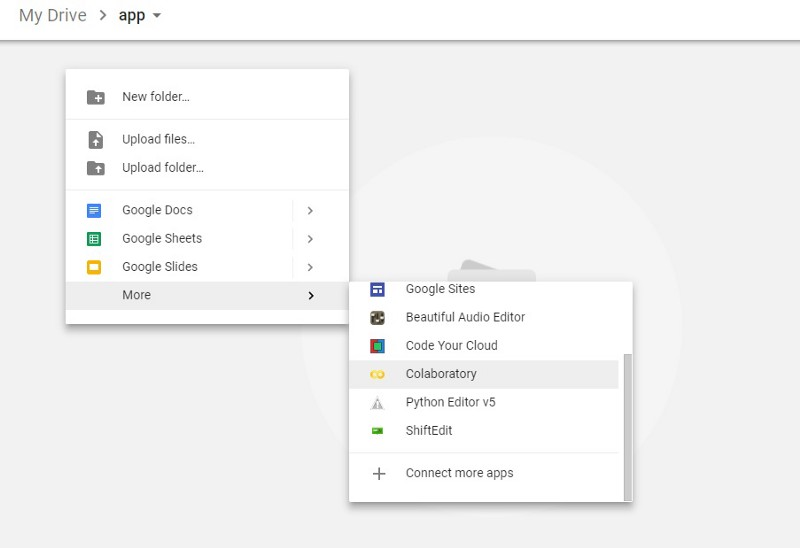
\includegraphics[width=0.8\textwidth]{colab_settings_1.jpeg}
    \label{fig:colab_settings_1}
\end{figure}

\item В разделе \textsl{Runtime->Change runtime type} выбрать GPU
\begin{figure}[h]
    \centering
    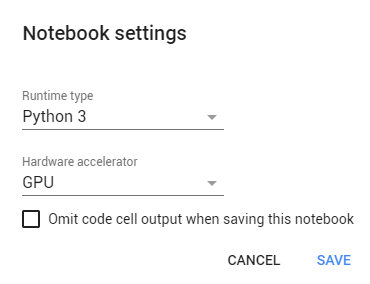
\includegraphics[width=0.6\textwidth]{colab_settings_2.png}
    \label{fig:colab_settings_2}
\end{figure}

\item На данном этапе уже можно использовать Google Colaboratory
\begin{figure}[h]
    \centering
    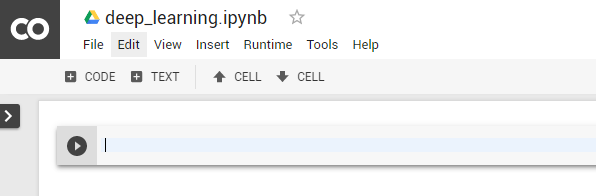
\includegraphics[width=0.85\textwidth]{colab_settings_3.png}
    \label{fig:colab_settings_3}
\end{figure}

\item Авторизуем учетную запись Google и подключим Google Drive следующими командами
\begin{figure}[h]
    \centering
    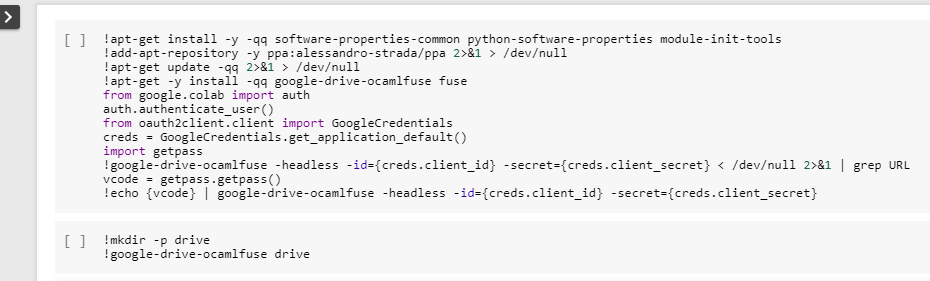
\includegraphics[width=0.85\textwidth]{colab_settings_4.png}
    \label{fig:colab_settings_4}
\end{figure}

\end{enumerate}

Теперь можно производить вычисления нa видеокарте NVIDIA Tesla K80 и взаимодействовать с Google Drive.

\newpage 